\subsection{FLOps' Local Data Management Architecture}
\begin{figure}[h]
    \begin{adjustwidth}{-0.1\paperwidth}{-0.1\paperwidth}
        \centering
        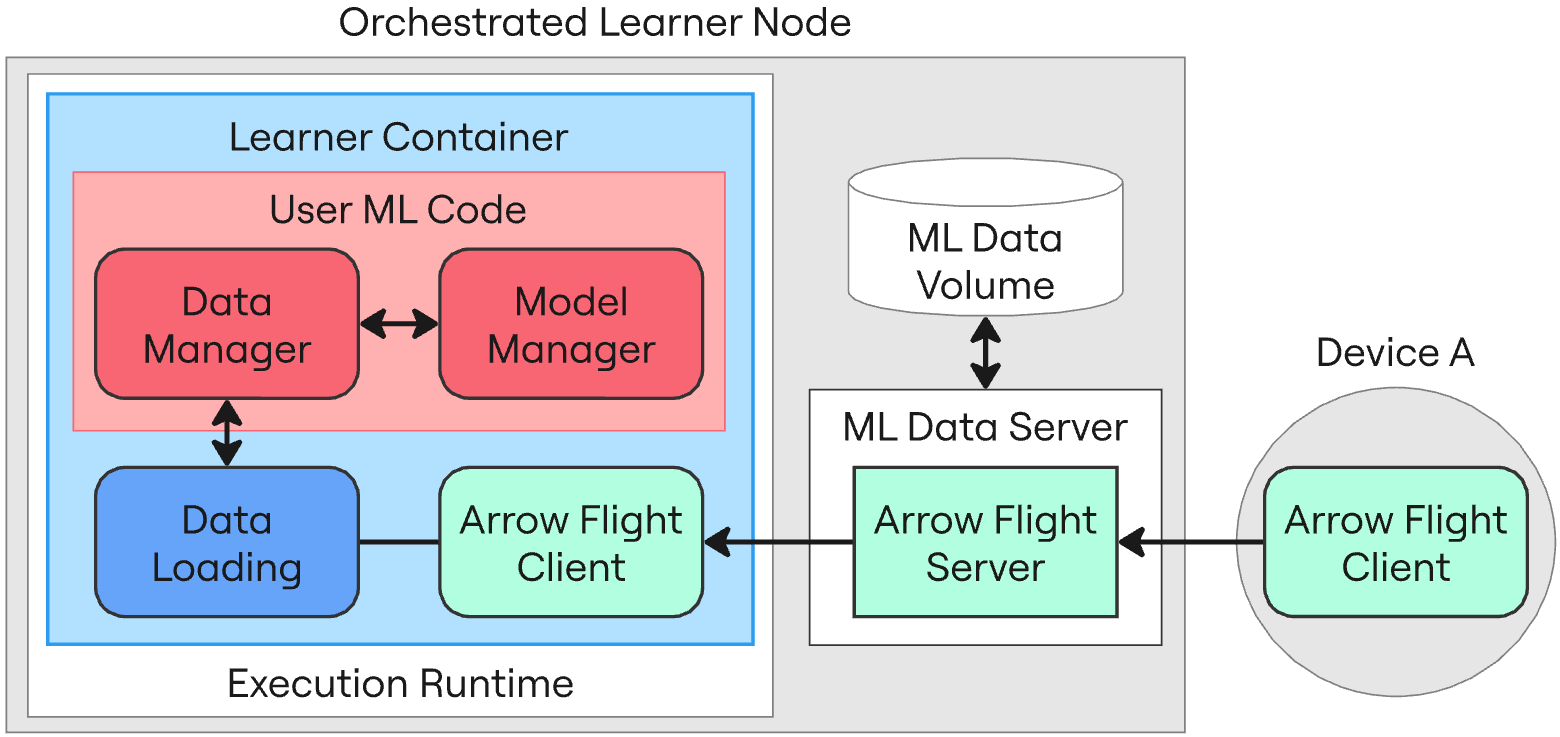
\includegraphics[width=0.80\paperwidth]{local_data_loading_medium.png}
        \caption{FLOps Local Data Management Structure}
        \label{fig:medium_local_data_management}
    \end{adjustwidth}
\end{figure}
Figure \ref{fig:medium_local_data_management} depicts the architecture of FLOps' local data management.
The important concretions compared to the simplified version in Figure \ref{fig:flops_simple_data_management} from \ref{subsection:flops_overview} are as follows:
The learner container and the data-providing device must have an Arrow Flight client installed and connected to the Arrow Flight server in the ML data server.
The data loading component in the learner uses the Flight client to retrieve the matching data.
It gets added by the builder service and is not part of the user's ML code.
The data and model manager utilize this loaded data.
Note that the figures in this subsection depict a single data source device for optimizing page space.
Arbitrary many devices are supported by this setup.

\begin{figure}[p]
    \begin{adjustwidth}{-0.1\paperwidth}{-0.1\paperwidth}
        \centering
        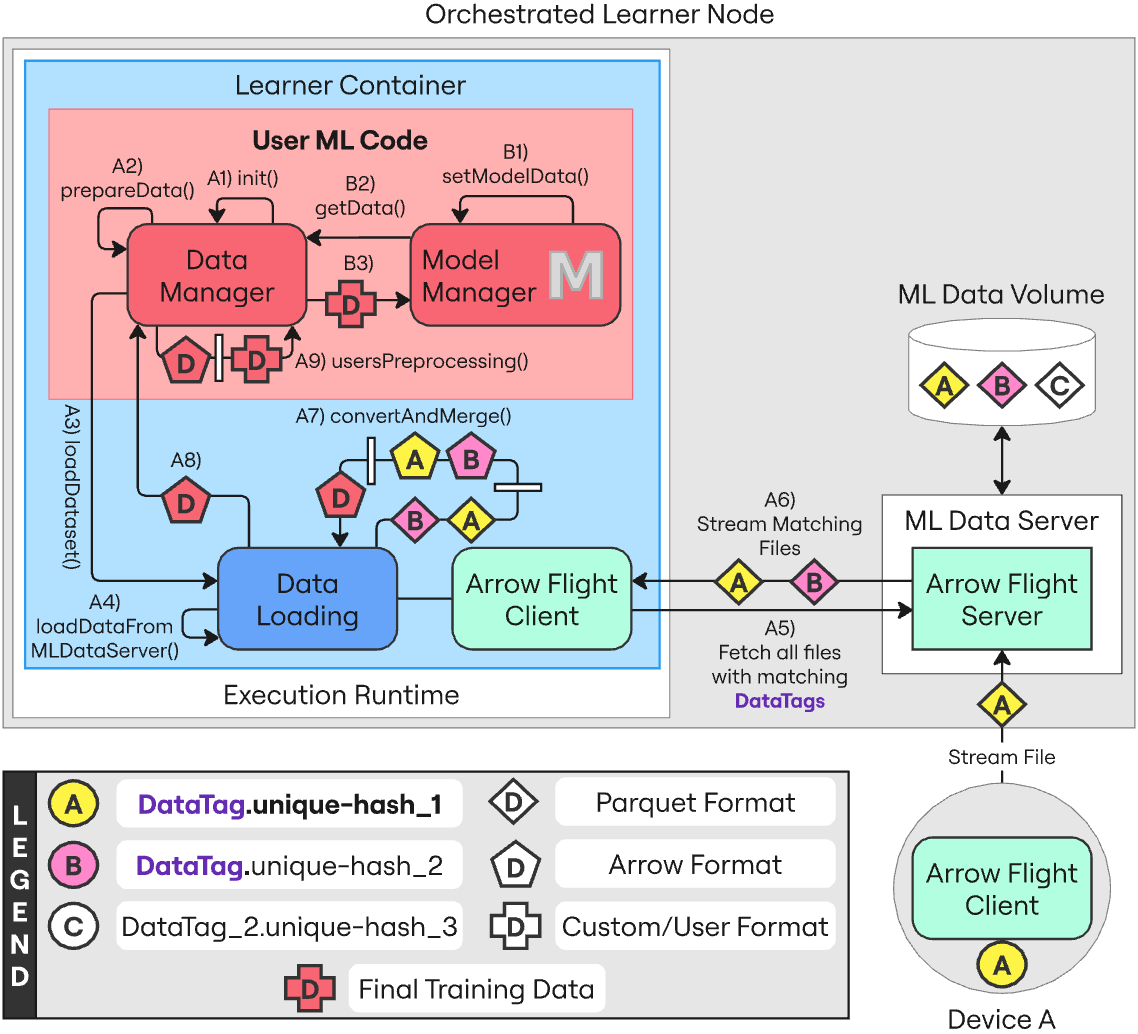
\includegraphics[width=0.90\paperwidth]{local_data_loading_detailed.png}
        \caption{Detailed FLOps Local Data Management Structure}
        \label{fig:detailed_local_data_management}
    \end{adjustwidth}
\end{figure}
Figure \ref{fig:detailed_local_data_management} depicts FLOps' local data management processes in more detail.
Firstly, the unique data resides on device A.
The device can store its data in an arbitrary format.
The device trusts the learner node in its proximity and transfers its data A to its ML data server via Flight.
For this, it needs to convert its data into Parquet format.
Secondly, the ML data server receives this streamed data and stores it locally on the learner node in a dedicated ML data volume.
This volume now contains several different Parquet files from different sources.
It uses Parquet files based on the last subsection's recommendations.

The next sequence of steps starts from the user's data manager.
During its initialization (A1), when the learner service is run, it triggers its \texttt{prepareData} function (A2).
This method calls the wrapper/adapter function \texttt{loadDataset} (A3).
The \texttt{loadDataset} function calls the \texttt{loadDataFromMLDataServer} function (A4).
This function is not available for users during development.
It is instead injected by the builder service, so it is exclusively available in the learner image's augmented FL code.

The Data Loading's \texttt{loadDataFromMLDataServer} function contacts its Flight client to request all matching files from the local ML data server (A5).
The match is performed based on the user's project SLA.
This SLA includes a \texttt{dataTags} key that is a list of string tags.
When devices send over their files, they must provide a data tag.
The ML data server will store these data files in the format seen in the Figure's legend.
The name starts with a singular data tag and ends with a unique hash based on the file's content.
Users and data providers need to cooperate to ensure that these data tags match.
The ML data server takes all files which name's prefix matches the user requested SLA data tags and streams them over into the learner container (A6).
In the example shown, only data files A and B have matching data tags.
The Flight server streams both over to the data-loading component.

Now that the matching data files are available inside the learner container, they must be transformed to fit the user's needs.
The data loading component converts its received Parquet files into Arrow format (A7) for better in-memory data management.
Usually, ML code expects and works with whole datasets instead of multiple split ones.
For this reason, the data loading component also merges its received files into a single dataset (A7).
The data loading component then sends this dataset to the user's data manager (A8).
The data manager now has access to the necessary dataset and can perform custom preprocessing and transformation steps (A9).
Users can freely configure and implement this preprocessing to ensure the retrieved data is usable for their ML model.

When FL training starts, the user's model manager will initially set the model data (B1).
Its \texttt{getData} method (B2) contacts the data manager and returns its prepared compatible dataset (B3).
In conclusion, these steps enable FLOps to manage and provide real local FL data to diverse user ML code for training and evaluation.